\documentclass{article}
\usepackage{amsmath}
\usepackage{amssymb}
\usepackage{graphicx}
\newcommand*{\QED}{\hfill\ensuremath{\blacksquare}}
\graphicspath{{.}}

\title{Computational Linear Algebra, Module 4}
\author{Maya Shende}
\date{Due: February 21st, 2018}

\begin{document}
\maketitle
	
\begin{enumerate}
	\item image:
	
	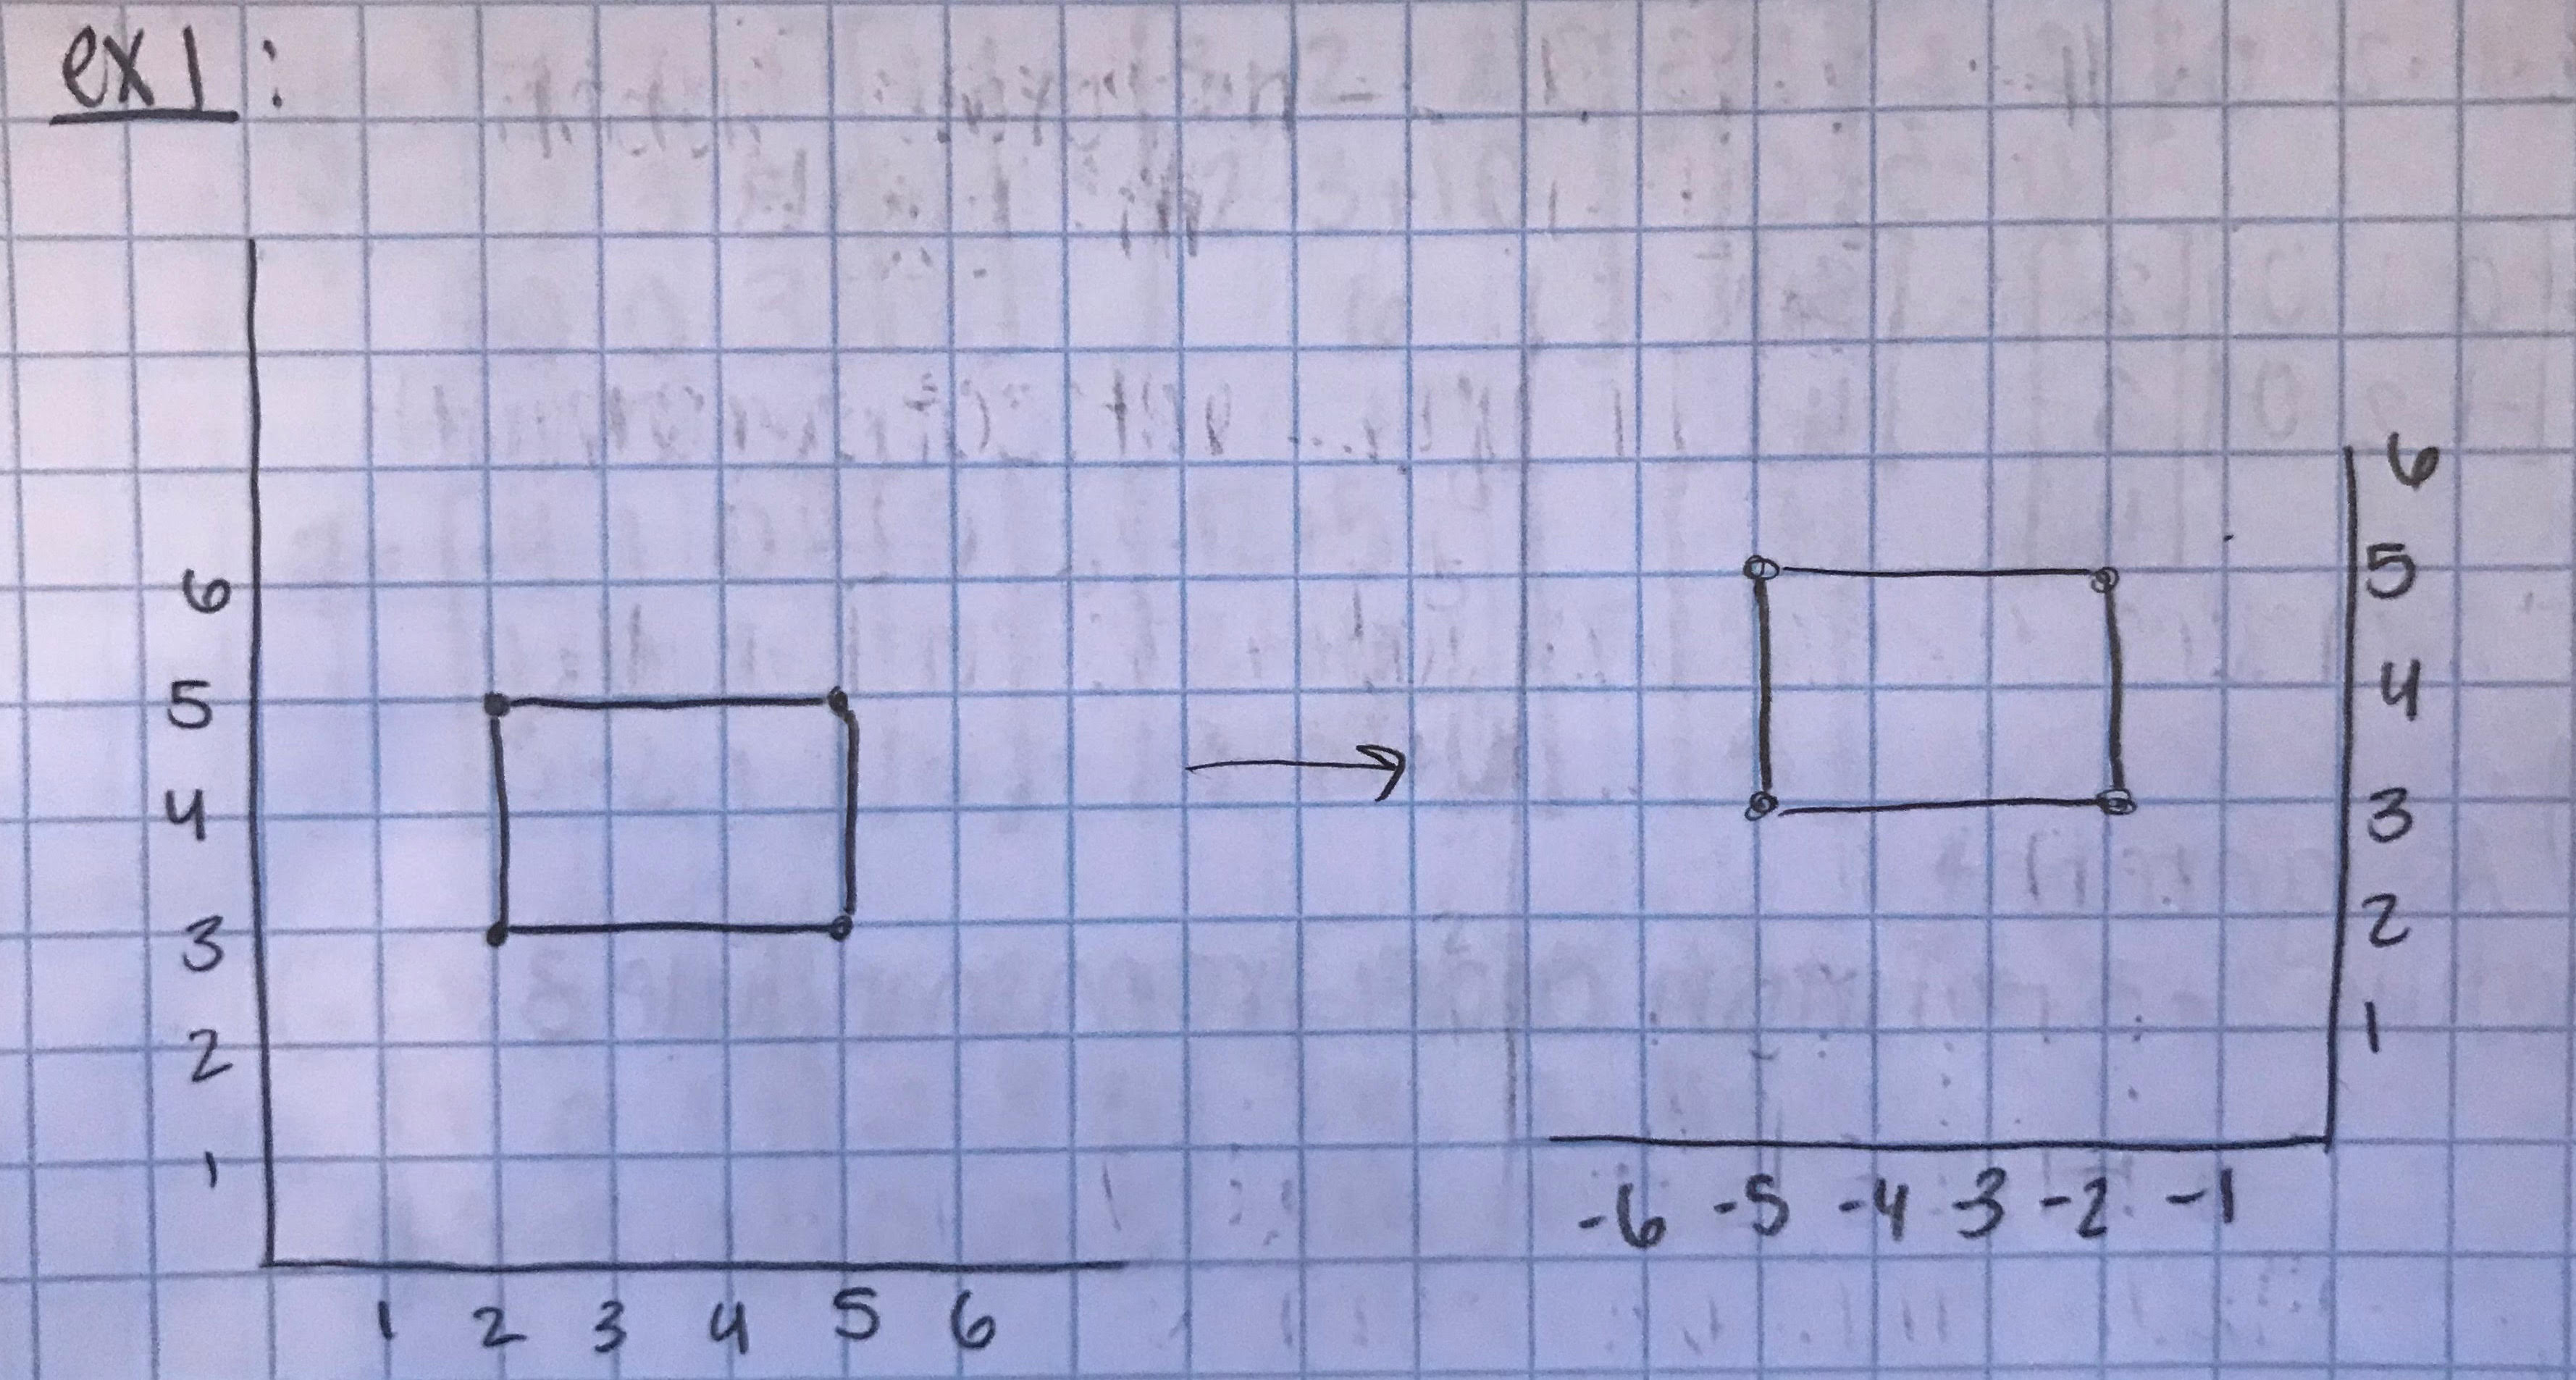
\includegraphics[scale=0.1]{exercise1}
	
	
	\item See code.
	
	\item $
	\begin{bmatrix}
		1	&0\\
		0	&-1
	\end{bmatrix}
	$ would result in reflecting a shape about the x-axis. 
	
	\item image:
	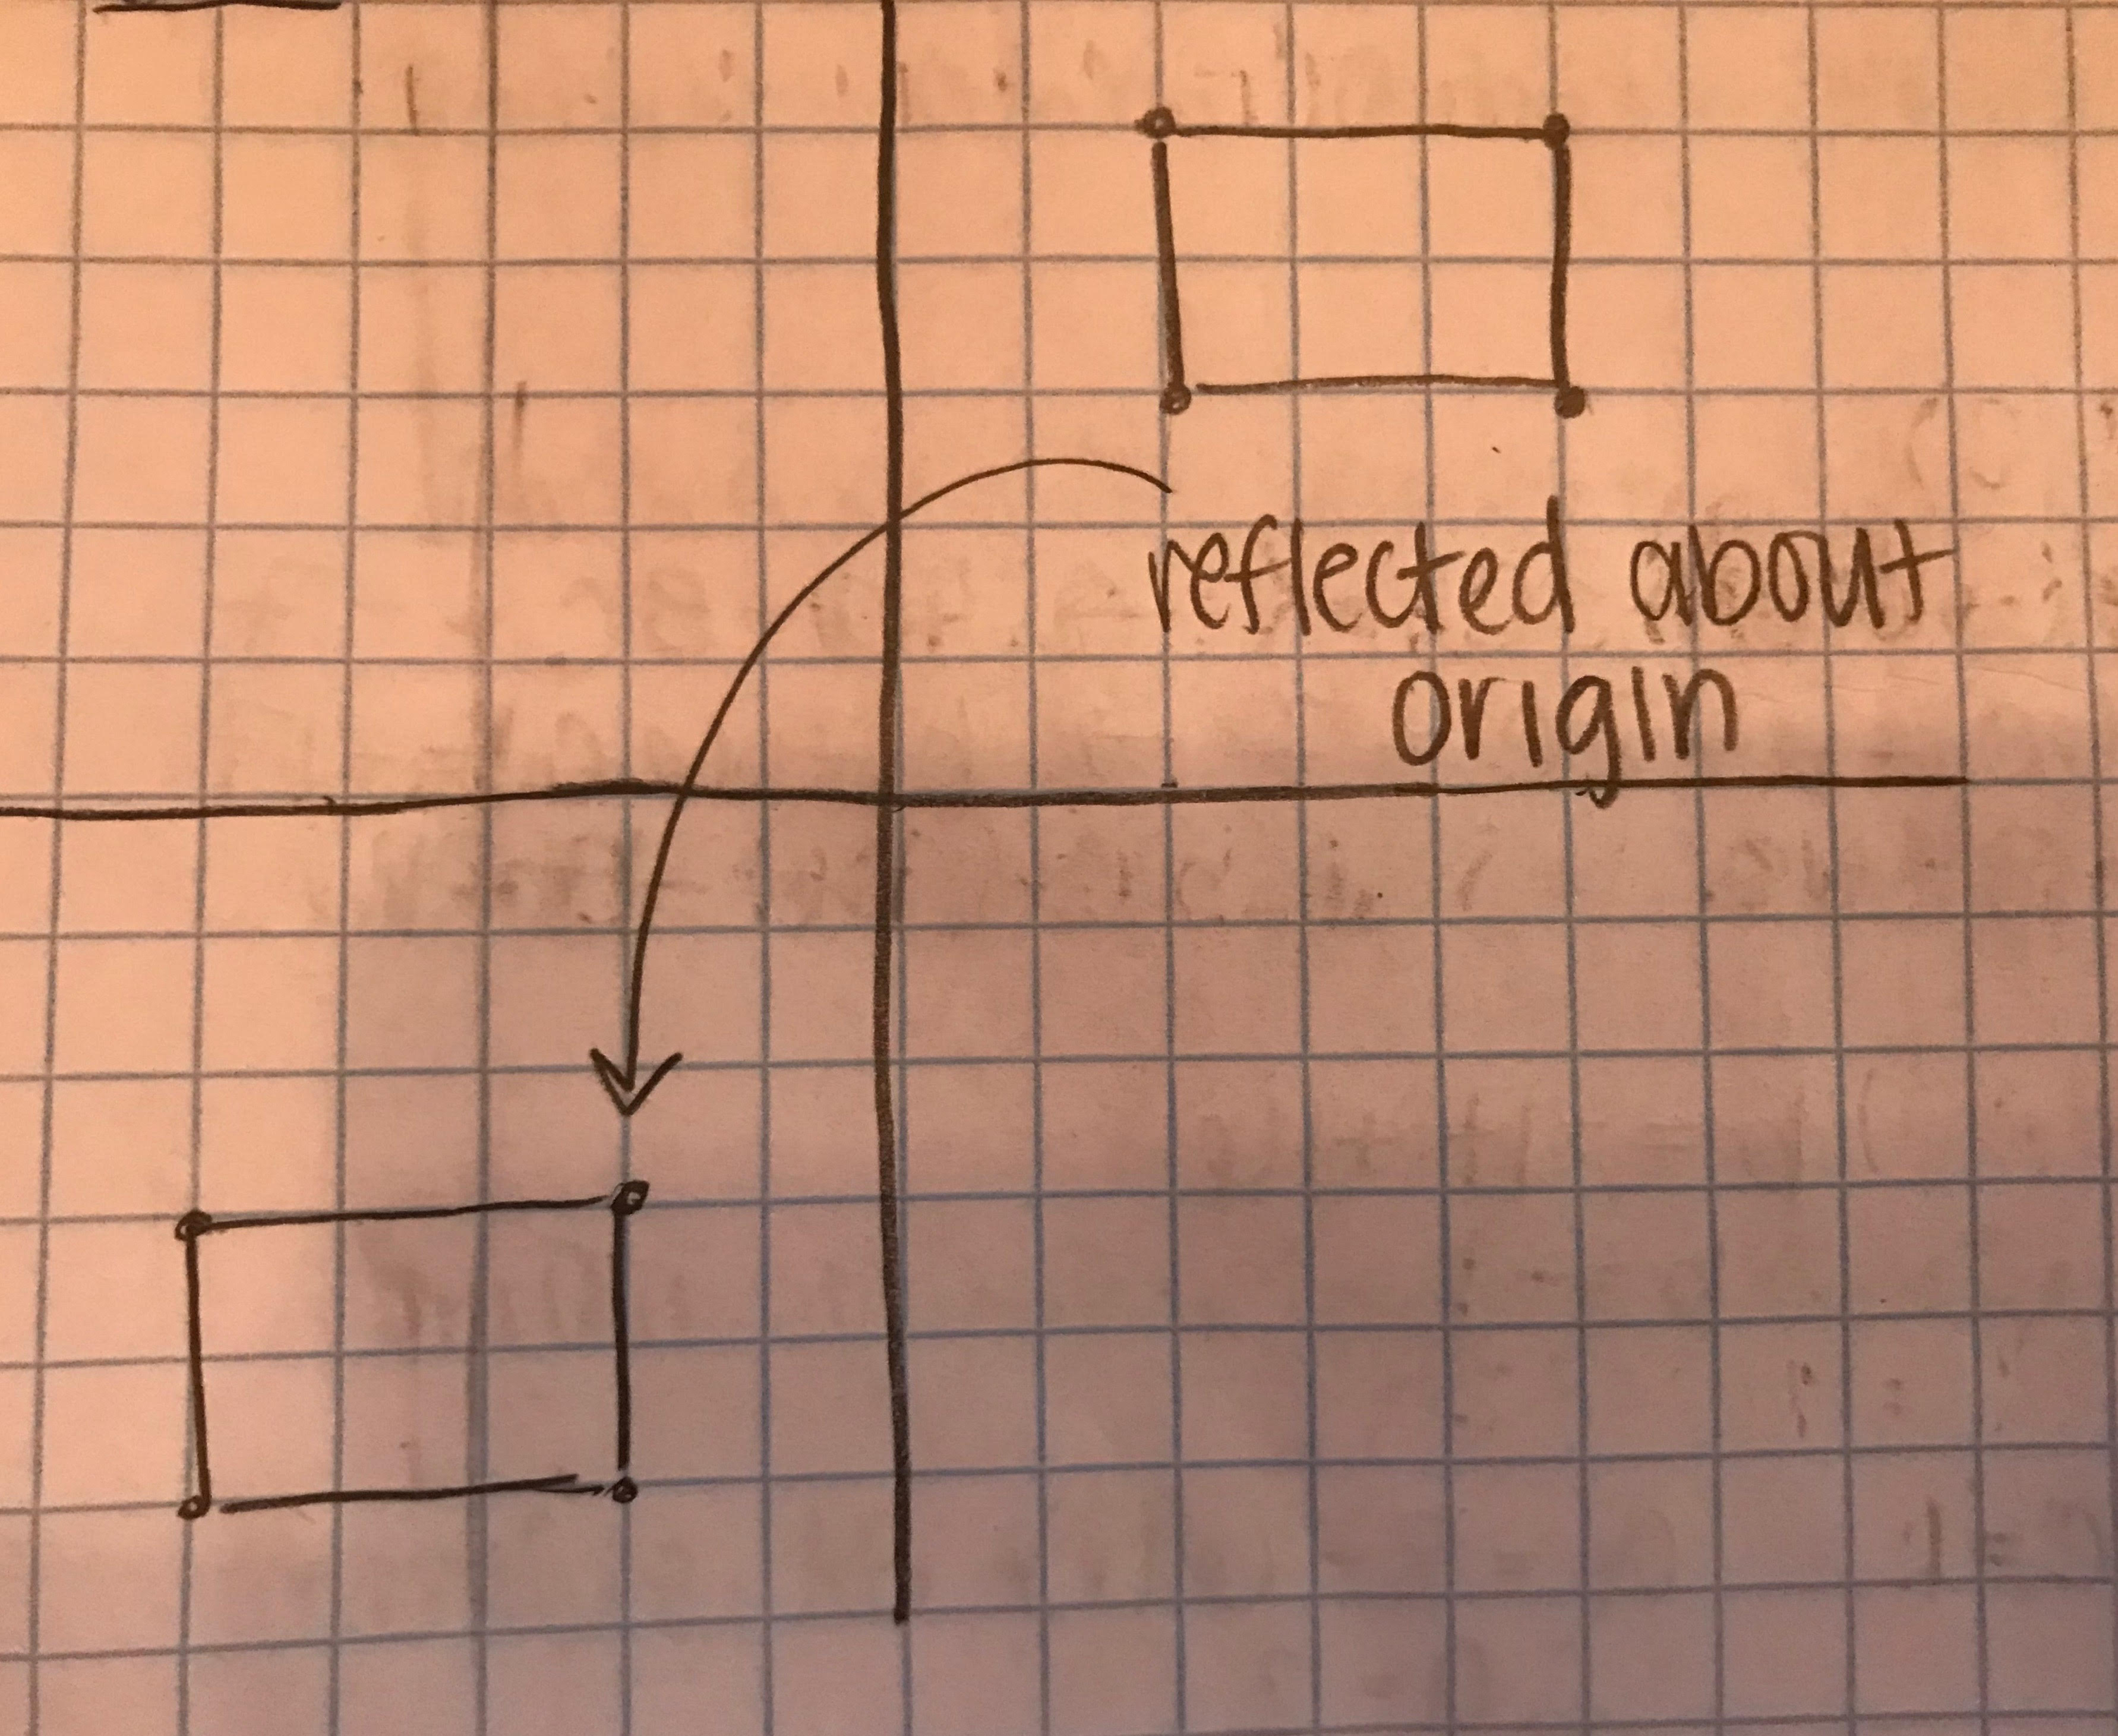
\includegraphics[scale=0.05]{exercise4}
	
	\item See code. 
	
	\item $BA = 
	\begin{bmatrix}
		-1	&0\\
		0	&-1
	\end{bmatrix}
	\begin{bmatrix}
		-1	&0\\
		0	&1
	\end{bmatrix}
	= 
	\begin{bmatrix}
		1	&0\\
		0	&-1
	\end{bmatrix}
	$. This is a reflection about the x-axis, which is what we would expect since we are first reflecting about the y-axis and then rotating about the origin. 
	
	\item We need the associativity property.
	
	\item When we change the order, nothing changes about the result. We have $AB = 
	\begin{bmatrix}
	-1	&0\\
	0	&1
	\end{bmatrix}
	\begin{bmatrix}
		-1	&0\\
		0	&-1
	\end{bmatrix}
	= 
	\begin{bmatrix}
		1	&0\\
		0	&-1
	\end{bmatrix}
	$. This makes it seem like the multiplication of matrices is commutative. Geometrically, this just means that the two transformations we performed do commute with each other. 

	\item This transformation looks like a rotation about some point other than the origin.
	
	\item In this case, the order of the transformations does matter - this is because there is some rotation involved. 
	
	\item This transformation effectively puts the rectangle where it was originally. This means that the matrix B is just rotating the rectangle by some amount when used alone. If we apply C to a vector v, we will see that v will remain unchanged. 
	
	\item 

Prove $\textbf{AB} \neq \textbf{BA} $:
		$$	\text{Let } 
		\textbf{A} = \begin{bmatrix}
		a_{11}  & a_{12} & ... & a_{1i} & ... & a_{1n} \\
		a_{21}  & a_{22} & ... & a_{2i} & ... & a_{n2} \\
		...    &  ...   & ... &  ...   & ... & ...    \\
		a_{j1}  & a_{j2} & ... & a_{ji} & ... & a_{nj} \\
		...    &  ...   & ... &  ...   & ... & ...    \\
		a_{m1}  & a_{m2} & ... & a_{mi} & ... & a_{mn} 
		\end{bmatrix}  
		\text{and }
		\textbf{B} = \begin{bmatrix}
		b_{11}  & b_{12} & ... & b_{1i} & ... & b_{1n} \\
		b_{21}  & b_{22} & ... & b_{2i} & ... & b_{n2} \\
		...    &  ...   & ... &  ...   & ... & ...    \\
		b_{j1}  & b_{j2} & ... & b_{ji} & ... & b_{nj} \\
		...    &  ...   & ... &  ...   & ... & ...    \\
		b_{m1}  & b_{m2} & ... & b_{mi} & ... & b_{mn} 
		\end{bmatrix}$$
		
		Then, 
		$$\textbf{AB} = \begin{bmatrix}
		a_{11}  & a_{12} & ... & a_{1i} & ... & a_{1n} \\
		a_{21}  & a_{22} & ... & a_{2i} & ... & a_{2n} \\
		...    &  ...   & ... &  ...   & ... & ...    \\
		a_{j1}  & a_{j2} & ... & a_{ji} & ... & a_{jn} \\
		...    &  ...   & ... &  ...   & ... & ...    \\
		a_{n1}  & a_{n2} & ... & a_{ni} & ... & a_{nn} 
		\end{bmatrix} \begin{bmatrix}
		b_{11}  & b_{12} & ... & b_{1i} & ... & b_{1n} \\
		b_{21}  & b_{22} & ... & b_{2i} & ... & b_{2n} \\
		...    &  ...   & ... &  ...   & ... & ...    \\
		b_{j1}  & b_{j2} & ... & b_{ji} & ... & b_{jn} \\
		...    &  ...   & ... &  ...   & ... & ...    \\
		b_{n1}  & b_{n2} & ... & b_{ni} & ... & b_{nn}
		\end{bmatrix} $$

		$$= \begin{bmatrix}
		a_{11} b_{11} + ... + a_{1n} b_{n1}  & a_{11} b_{12} + ... + a_{1n} b_{n2} & ... & a_{11} b_{1i} + ... + a_{1n} b_{ni} & ... & a_{11} b_{1n} + ... + a_{1n} b_{nn} \\
		a_{21} b_{11} + ... + a_{2n} b_{n1}  & a_{21} b_{12} + ... + a_{2n} b_{n2} & ... & a_{21} b_{2i} + ... + a_{2n} b_{ni} & ... & a_{21} b_{2n} + ... + a_{2n} b_{nn} \\
		...       &      ...      & ... &      ...      & ... &      ...      \\
		a_{j1} b_{11} + ... + a_{jn} b_{n1}  & a_{j1} b_{12} + ... + a_{jn} b_{n2} & ... & a_{j1} b_{1i} + ... + a_{jn} b_{ni} & ... & a_{j1} b_{1n} + ... + a_{jn} b_{nn} \\
		...       &      ...      & ... &      ...      & ... &      ...      \\
		a_{n1} b_{11} + ... + a_{nn} b_{n1}  & a_{n1} b_{12} + ... + a_{nn} b_{n2} & ... & a_{n1} b_{1i} + ... + a_{nn} b_{ni} & ... & a_{n1} b_{1n} + ... + a_{nn} b_{nn} 
		\end{bmatrix}$$
		
		
		and 
		$$\textbf{BA} = \begin{bmatrix} 
		b_{11}  & b_{12} & ... & b_{1i} & ... & b_{1n} \\
		b_{21}  & b_{22} & ... & b_{2i} & ... & b_{2n} \\
		...    &  ...   & ... &  ...   & ... & ...    \\
		b_{j1}  & b_{j2} & ... & b_{ji} & ... & b_{jn} \\
		...    &  ...   & ... &  ...   & ... & ...    \\
		b_{n1}  & b_{n2} & ... & b_{ni} & ... & b_{nn}
		\end{bmatrix} \begin{bmatrix}
		a_{11}  & a_{12} & ... & a_{1i} & ... & a_{1n} \\
		a_{21}  & a_{22} & ... & a_{2i} & ... & a_{2n} \\
		...    &  ...   & ... &  ...   & ... & ...    \\
		a_{j1}  & a_{j2} & ... & a_{ji} & ... & a_{jn} \\
		...    &  ...   & ... &  ...   & ... & ...    \\
		a_{n1}  & a_{n2} & ... & a_{ni} & ... & a_{nn}
		\end{bmatrix} $$
	
		$$= \begin{bmatrix}
		b_{11} a_{11} + ... + b_{1n} a_{n1}  & b_{11} a_{12} + ... + b_{1n} a_{n2} & ... & b_{11} a_{1i} + ... + b_{1n} a_{ni} & ... & b_{11} a_{1n} + ... + b_{1n} a_{nn} \\
		b_{21} a_{11} + ... + b_{2n} a_{n1}  & b_{21} a_{12} + ... + b_{2n} a_{n2} & ... & b_{21} a_{2i} + ... + b_{2n} a_{ni} & ... & b_{21} a_{2n} + ... + b_{2n} a_{nn} \\
		...       &      ...      & ... &      ...      & ... &      ...      \\
		b_{j1} a_{11} + ... + b_{jn} a_{n1}  & b_{j1} a_{12} + ... + b_{jn} a_{n2} & ... & b_{j1} a_{1i} + ... + b_{jn} a_{ni} & ... & b_{j1} a_{1n} + ... + b_{jn} a_{nn} \\
		...       &      ...      & ... &      ...      & ... &      ...      \\
		b_{n1} a_{11} + ... + b_{nn} a_{n1}  & b_{n1} a_{12} + ... + b_{nn} a_{n2} & ... & b_{n1} a_{1i} + ... + b_{nn} a_{ni} & ... & b_{n1} a_{1n} + ... + b_{nn} a_{nn} 
		\end{bmatrix}$$
		
	Since, $b_{j1} a_{12} + ... + b_{jn} a_{n2} \neq a_{j1} b_{12} + ... + a_{jn} b_{n2}$ therefore \textbf{AB} $\neq$ \textbf{BA} \QED \\
	 
	Prove $ \textbf{A}(\textbf{BC}) = (\textbf{AB})\textbf{C} $:
		$$	\text{Let } 
		\textbf{A} = \begin{bmatrix}
		a_{11}  &  ... & a_{1n} \\
		a_{21}  &  ... & a_{2n} \\
		...     &  ... & ...    \\
		a_{m1}  &  ... & a_{mn} 
		\end{bmatrix}  
		\text{and }
		\textbf{B} = \begin{bmatrix}
		b_{11}  &  ... & b_{1n} \\
		b_{21}  &  ... & b_{2n} \\
		...     &  ... & ...    \\
		b_{m1}  &  ... & b_{mn}
		\end{bmatrix}
		\text{and }
		\textbf{C} = \begin{bmatrix}
		c_{11}  &  ... & c_{1n} \\
		c_{21}  &  ... & c_{2n} \\
		...     &  ... & ...    \\
		c_{m1}  &  ... & c_{mn}
		\end{bmatrix}$$
		
		Then, 
		$$\textbf{A(BC)} = \begin{bmatrix}
		a_{11}  &  ... & a_{1n} \\
		a_{21}  &  ... & a_{2n} \\
		...     &  ... & ...    \\
		a_{m1}  &  ... & a_{mn} 
		\end{bmatrix}
		\left(
		\begin{bmatrix}
		b_{11}  &  ... & b_{1n} \\
		b_{21}  &  ... & b_{2n} \\
		...     &  ... & ...    \\
		b_{m1}  &  ... & b_{mn}
		\end{bmatrix} \begin{bmatrix}
		c_{11}  &  ... & c_{1n} \\
		c_{21}  &  ... & c_{2n} \\
		...     &  ... & ...    \\
		c_{m1}  &  ... & c_{mn}
		\end{bmatrix}\right)$$
		
		$$= \begin{bmatrix}
		a_{11}  &  ... & a_{1n} \\
		a_{21}  &  ... & a_{2n} \\
		...     &  ... & ...    \\
		a_{m1}  &  ... & a_{mn} 
		\end{bmatrix}
		\left(
		\begin{bmatrix}
		b_{11} c_{11} + ... + b_{1n} c_{m1} & ... & b_{11} c_{1n} + ... + b_{1n} c_{mn} \\
		b_{21} c_{11} + ... + b_{2n} c_{m1} & ... & b_{21} c_{1n} + ... + b_{2n} c_{mn} \\
		...       &      ...      &      ...      \\
		b_{m1} c_{11} + ... + b_{mn} c_{m1}  & ... & b_{m1} c_{1n} + ... + b_{mn} c_{mn}
		\end{bmatrix}\right)$$
		
		$$= \begin{bmatrix}
		a_{11} (b_{11} c_{11} + ... + b_{1n} c_{m1}) + ...  & ... & a_{11} (b_{m1} c_{11} + ... + b_{mn} c_{m1}) + ... \\
		...       &      ...      &      ...      \\
		a_{m1} (b_{11} c_{11} + ... + b_{1n} c_{m1}) + ...  & ... & a_{m1} (b_{m1} c_{11} + ... + b_{mn} c_{m1}) + ... \\
		\end{bmatrix}$$
		
		$$= \left(\begin{bmatrix}
		a_{11} b_{11} + ... + a_{1n} b_{m1} & ... & a_{11} b_{1n} + ... + a_{1n} b_{mn} \\
		a_{21} b_{11} + ... + a_{2n} b_{m1} & ... & a_{21} b_{1n} + ... + a_{2n} b_{mn} \\
		...       &      ...      &      ...      \\
		a_{m1} b_{11} + ... + a_{mn} b_{m1}  & ... & a_{m1} b_{1n} + ... + a_{mn} b_{mn}
		\end{bmatrix}\right) \begin{bmatrix}
		c_{11}  &  ... & c_{1n} \\
		c_{21}  &  ... & c_{2n} \\
		...     &  ... & ...    \\
		c_{m1}  &  ... & c_{mn}
		\end{bmatrix} $$
		
		$$ = \left( \begin{bmatrix}
		a_{11}  &  ... & a_{1n} \\
		a_{21}  &  ... & a_{2n} \\
		...     &  ... & ...    \\
		a_{m1}  &  ... & a_{mn} 
		\end{bmatrix} \begin{bmatrix}
		b_{11}  &  ... & b_{1n} \\
		b_{21}  &  ... & b_{2n} \\
		...     &  ... & ...    \\
		b_{m1}  &  ... & b_{mn}
		\end{bmatrix}\right) \begin{bmatrix}
		c_{11}  &  ... & c_{1n} \\
		c_{21}  &  ... & c_{2n} \\
		...     &  ... & ...    \\
		c_{m1}  &  ... & c_{mn}
		\end{bmatrix}$$
		
		Therefore, $ \textbf{A}(\textbf{BC}) = (\textbf{AB})\textbf{C} $ \QED \\
		
	Prove $ \textbf{A}(\textbf{B} + \textbf{C}) = (\textbf{AB})+(\textbf{CB}) $:
		$$	\text{Let } 
		\textbf{A} = \begin{bmatrix}
		a_{11}  &  ... & a_{1n} \\
		a_{21}  &  ... & a_{2n} \\
		...     &  ... & ...    \\
		a_{m1}  &  ... & a_{mn} 
		\end{bmatrix}  
		\text{and }
		\textbf{B} = \begin{bmatrix}
		b_{11}  &  ... & b_{1n} \\
		b_{21}  &  ... & b_{2n} \\
		...     &  ... & ...    \\
		b_{m1}  &  ... & b_{mn}
		\end{bmatrix}
		\text{and }
		\textbf{C} = \begin{bmatrix}
		c_{11}  &  ... & c_{1n} \\
		c_{21}  &  ... & c_{2n} \\
		...     &  ... & ...    \\
		c_{m1}  &  ... & c_{mn}
		\end{bmatrix}$$
		
		Then, 
		$$\textbf{A(B+C)} = \begin{bmatrix}
		a_{11}  &  ... & a_{1n} \\
		a_{21}  &  ... & a_{2n} \\
		...     &  ... & ...    \\
		a_{m1}  &  ... & a_{mn} 
		\end{bmatrix}
		\left(
		\begin{bmatrix}
		b_{11}  &  ... & b_{1n} \\
		b_{21}  &  ... & b_{2n} \\
		...     &  ... & ...    \\
		b_{m1}  &  ... & b_{mn}
		\end{bmatrix} + \begin{bmatrix}
		c_{11}  &  ... & c_{1n} \\
		c_{21}  &  ... & c_{2n} \\
		...     &  ... & ...    \\
		c_{m1}  &  ... & c_{mn}
		\end{bmatrix}\right)$$
		
		$$= \begin{bmatrix}
		a_{11}  &  ... & a_{1n} \\
		a_{21}  &  ... & a_{2n} \\
		...     &  ... & ...    \\
		a_{m1}  &  ... & a_{mn} 
		\end{bmatrix}
		\left(
		\begin{bmatrix}
		b_{11} + c_{11}  &  ... & b_{1n} + c_{1n} \\
		b_{21} + c_{21}  &  ... & b_{2n} + c_{2n} \\
		...     &  ... & ...    \\
		b_{m1} + c_{m1}  &  ... & b_{mn} + c_{mn}
		\end{bmatrix}\right)$$
		
		$$= \begin{bmatrix}
		a_{11}(b_{11} + c_{11}) + ... + a_{1n}(b_{m1} + c_{m1}) & ... & a_{11}(b_{1n} + c_{1n}) + ... + a_{1n}(b_{mn} + c_{mn}) \\
		a_{21}(b_{11} + c_{11}) + ... + a_{2n}(b_{m1} + c_{m1}) & ... & a_{21}(b_{1n} + c_{1n}) + ... + a_{2n}(b_{mn} + c_{mn}) \\
		... & ... & ... \\
		a_{m1}(b_{11} + c_{11}) + ... + a_{mn}(b_{m1} + c_{m1}) & ... & a_{m1}(b_{1n} + c_{1n}) + ... + a_{mn}(b_{mn} + c_{mn}) \\
		\end{bmatrix}$$
		
		$$= \begin{bmatrix}
		(a_{11}b_{11} + a_{11}c_{11}) + ... + (a_{1n}b_{m1} + a_{1n}c_{m1}) & ... & (a_{11}b_{1n} + a_{11}c_{1n}) + ... + (a_{1n}b_{mn} + a_{1n}c_{mn}) \\
		(a_{21}b_{11} + a_{21}c_{11}) + ... + (a_{2n}b_{m1} + a_{2n}c_{m1}) & ... & (a_{21}b_{1n} + a_{21}c_{1n}) + ... + (a_{2n}b_{mn} + a_{2n}c_{mn}) \\
		... & ... & ... \\
		(a_{m1}b_{11} + a_{m1}c_{11}) + ... + (a_{mn}b_{m1} + a_{mn}c_{m1}) & ... & (a_{m1}b_{1n} + a_{m1}c_{1n}) + ... + (a_{mn}b_{mn} + a_{mn}c_{mn}) \\
		\end{bmatrix}$$
		
		$$= \begin{bmatrix}
		a_{11}b_{11} + ... + a_{1n}b_{m1} & ... & a_{11}b_{1n} + ... + a_{1n}b_{mn} \\
		a_{21}b_{11} + ... + a_{2n}b_{m1} & ... & a_{21}b_{1n} + ... + a_{2n}b_{mn} \\
		... & ... & ... \\
		a_{m1}b_{11} + ... + a_{mn}b_{m1} & ... & a_{m1}b_{1n} + ... + a_{mn}b_{mn} \\
		\end{bmatrix}$$ $$ \hspace{2cm} + \begin{bmatrix}
		a_{11}c_{11} + ... + a_{1n}c_{m1} & ... & a_{11}c_{1n} + ... + a_{1n}c_{mn} \\
		a_{21}c_{11} + ... + a_{2n}c_{m1} & ... & a_{21}c_{1n} + ... + a_{2n}c_{mn} \\
		... & ... & ... \\
		a_{m1}c_{11} + ... + a_{mn}c_{m1} & ... & a_{m1}c_{1n} + ... + a_{mn}c_{mn}
		\end{bmatrix}$$
		
		Therefore, $ \textbf{A}(\textbf{B} + \textbf{C}) = (\textbf{AB})+(\textbf{CB}) $ \QED \\
	
	Prove $ \alpha (\textbf{AB}) = (\alpha\textbf{A})\textbf{B} $:
		$$	\text{Let } 
		\textbf{A} = \begin{bmatrix}
		a_{11}  &  ... & a_{1n} \\
		a_{21}  &  ... & a_{2n} \\
		...     &  ... & ...    \\
		a_{m1}  &  ... & a_{mn} 
		\end{bmatrix}  
		\text{and }
		\textbf{B} = \begin{bmatrix}
		b_{11}  &  ... & b_{1n} \\
		b_{21}  &  ... & b_{2n} \\
		...     &  ... & ...    \\
		b_{m1}  &  ... & b_{mn}
		\end{bmatrix}$$
		
		Then, 
		$$\alpha (\textbf{AB}) = \alpha \left( \begin{bmatrix}
		a_{11}  &  ... & a_{1n} \\
		a_{21}  &  ... & a_{2n} \\
		...     &  ... & ...    \\
		a_{m1}  &  ... & a_{mn} 
		\end{bmatrix} \begin{bmatrix}
		b_{11}  &  ... & b_{1n} \\
		b_{21}  &  ... & b_{2n} \\
		...     &  ... & ...    \\
		b_{m1}  &  ... & b_{mn}
		\end{bmatrix} \right)$$
		
		$$= \alpha \begin{bmatrix}
		a_{11} b_{11} + ... + a_{1n} b_{m1} & ... & a_{11} b_{1n} + ... + a_{1n} b_{mn} \\
		a_{21} b_{11} + ... + a_{2n} b_{m1} & ... & a_{21} b_{1n} + ... + a_{2n} b_{mn} \\
		...       &      ...      &      ...      \\
		a_{m1} b_{11} + ... + a_{mn} b_{m1}  & ... & a_{m1} b_{1n} + ... + a_{mn} b_{mn}
		\end{bmatrix} $$
		
		$$ = \begin{bmatrix}
		\alpha(a_{11} b_{11} + ... + a_{1n} b_{m1}) & ... & \alpha(a_{11} b_{1n} + ... + a_{1n} b_{mn}) \\
		\alpha(a_{21} b_{11} + ... + a_{2n} b_{m1}) & ... & \alpha(a_{21} b_{1n} + ... + a_{2n} b_{mn}) \\
		...       &      ...      &      ...      \\
		\alpha(a_{m1} b_{11} + ... + a_{mn} b_{m1})  & ... & \alpha(a_{m1} b_{1n} + ... + a_{mn} b_{mn})
		\end{bmatrix} $$
		
		$$ = \begin{bmatrix}
		(\alpha a_{11}) b_{11} + ... + (\alpha a_{1n}) b_{m1} & ... & (\alpha a_{11}) b_{1n} + ... + (\alpha a_{1n}) b_{mn} \\
		(\alpha a_{21}) b_{11} + ... + (\alpha a_{2n}) b_{m1} & ... & (\alpha a_{21}) b_{1n} + ... + (\alpha a_{2n}) b_{mn} \\
		...       &      ...      &      ...      \\
		(\alpha a_{m1}) b_{11} + ... + (\alpha a_{mn}) b_{m1}  & ... & (\alpha a_{m1}) b_{1n} + ... + (\alpha a_{mn}) b_{mn}
		\end{bmatrix} $$
		
		$$= \left( \alpha\begin{bmatrix}
		a_{11}  &  ... & a_{1n} \\
		a_{21}  &  ... & a_{2n} \\
		...     &  ... & ...    \\
		a_{m1}  &  ... & a_{mn} 
		\end{bmatrix}\right) \begin{bmatrix}
		b_{11}  &  ... & b_{1n} \\
		b_{21}  &  ... & b_{2n} \\
		...     &  ... & ...    \\
		b_{m1}  &  ... & b_{mn}
		\end{bmatrix} $$
		
		Therefore, $ \alpha (\textbf{AB}) = (\alpha\textbf{A})\textbf{B} $ \QED 
		
	\item I think more properties are needed for this proof, because none of the given properties say anything about the direction of multiplication, and we would need either some property stating something about direction of multiplication, or some sort of commutative property (which we know not to be true). 
	
	\item See code.
	
	\item The vectors $(0,1)$ and $(0,2)$ do not span the whole space of 2D vectors. This is because they are not linearly independent vectors. In 3D, an example of vectors that do not span all of 3D space is $(0,1,0)$, $(1,0,0)$ and $(1,2,0)$ since all of these vectors are in the $z=0$ plane. 
	
	\item No, you always need n vectors to span n-D space. 
	
	\item $(1,4) = (1,0) + 4(0,1) = e_1 + 4e_2$\\
	$(2,3) = 2(1,0) + 3(0,1) = 2e_1 + 3e_2$\\
	Yes, $e_1$ and $e_2$ span 2D space. 
	
	\item In standard coordinates, we see that $\cos{\theta} = \frac{x}{h}$ and $\sin{\theta} = \frac{u}{h}$. Similarly, we can get the coordinates for the other new axis.
	
	\item Clockwise rotation by $\theta$: $
	\begin{bmatrix}
		\cos{\theta}	&\cos{\theta}\\
		-\sin{\theta}	&\sin{\theta}
	\end{bmatrix}
	$\\
	Reflection about the x-axis: $
	\begin{bmatrix}
		1	&0\\
		0	&-1
	\end{bmatrix}
	$
	
	\item You can't derive a multiplicative matrix to do translations by using the above step-by-step approach. 
	
	\item Need to do still. 
	
	\item When $C$ is applied to a 2D vector, we get $
	\begin{bmatrix}
		c_{11}x + c_{12}y\\
		c_{21}x + c_{22}y
	\end{bmatrix}
	$. When the affine matrix for C is applied to the 3D affine vector for the original vector, we get $
	\begin{bmatrix}
		c_{11}x + c_{12}y\\
		c_{21}x + c_{22}y\\
		1	
	\end{bmatrix}
	$
	
	\item Need to do still.
	
	\item We will show this using 2x2 matrices (3x3 affine matrices). \\
	$affine(B) = 
	\begin{bmatrix}
		b_{11}	&b_{12}	&0\\
		b_{21}	&b_{22}	&0\\
		0	&0	&1
	\end{bmatrix}
	$ and $ affine(A) = 
	\begin{bmatrix}
		a_{11}	&a_{12}	&0\\
		a_{21}	&a_{22}	&0\\
		0	&0	&1	
	\end{bmatrix}
	$ and $ affine(u) = 
	\begin{bmatrix}
		u_1\\
		u_2\\
		1
	\end{bmatrix}
	$. So, $ affine(B) affine(A) = 
	\begin{bmatrix}
		b_{11}a_{11} + b_{12}a_{12}	&b_{11}a_{12} + b_{12}a_{22}	&0\\
		b_{21}a_{11} + b_{22}a_{12}	&b_{21}a_{12} + b_{22}a_{22}	&0\\
		0	&0	&1
	\end{bmatrix}
	\begin{bmatrix}
		u_1\\
		u_2\\
		1
	\end{bmatrix}
	= 
	\begin{bmatrix}
		u_1(b_{11}a_{11} + b_{12}a_{12})	&u_2(b_{11}a_{12} + b_{12}a_{22})	&0\\
		u_1(b_{21}a_{11} + b_{22}a_{12})	&u_2(b_{21}a_{12} + b_{22}a_{22})	&0\\
		0	&0	&1
	\end{bmatrix}
	$. Now, the projection of this is $
	\begin{bmatrix}
		u_1(b_{11}a_{11} + b_{12}a_{12})	&u_2(b_{11}a_{12} + b_{12}a_{22})\\
		u_1(b_{21}a_{11} + b_{22}a_{12})	&u_2(b_{21}a_{12} + b_{22}a_{22})
	\end{bmatrix}
	$ and this is the same as $BAu$. 
	
	\item See code.
	
	\item $AI = 
	\begin{bmatrix}
		a_{11}	&a_{12}	&\dots	&a_{1n}\\
		a_{21}	&a_{22}	&\dots	&a_{2n}\\
		\vdots	&\vdots	&\ddots	&\vdots\\
		a_{n1}	&a_{n2}	&\dots	&a_{nn}
	\end{bmatrix}
	\begin{bmatrix}
		1	&0	&\dots	&0\\
		0	&1	&\dots	&0\\
		\vdots	&\vdots	&\ddots	&\vdots\\
		0	&0	&\dots	&1	
	\end{bmatrix}
	= 
	\begin{bmatrix}
		a_{11}	&a_{12}	&\dots	&a_{1n}\\
		a_{21}	&a_{22}	&\dots	&a_{2n}\\
		\vdots	&\vdots	&\ddots	&\vdots\\
		a_{n1}	&a_{n2}	&\dots	&a_{nn}	
	\end{bmatrix}
	$. So, $AI = A$. For an m x n matrix, the identity matrix has to be an m x m square matrix.
	
	\item This is true because of how the matrix multiplication works. If we look at $Ab_i$, we will see that each of these sums (rows of A multiplied by the vector $b_i$) will equate to an entry in the vector $c_i$. 
	
	\item The undo matrix for reflection about the y-axis is $
	\begin{bmatrix}
		-1	&0\\
		0	&1
	\end{bmatrix}
	$. If we multiply the undo matrix with its original reflection matrix, we have $
	\begin{bmatrix}
		-1	&0\\
		0	&1
	\end{bmatrix}
	\begin{bmatrix}
		-1	&0\\
		0	&1		
	\end{bmatrix}
	= 
	\begin{bmatrix}
		1	&0\\
		0	&1		
	\end{bmatrix}
	$
	\item The undo matrix for translation by $p, q$ is $
	\begin{bmatrix}
		1	&0	&-p\\
		0	&1	&-q\\
		0	&0	&1
	\end{bmatrix}
	$. If we multiple the undo matrix with the original translation matrix, we have $
	\begin{bmatrix}
		1	&0	&p\\
		0	&1	&q\\
		0	&0	&1
	\end{bmatrix}	
	\begin{bmatrix}
		1	&0	&-p\\
		0	&1	&-q\\
		0	&0	&1
	\end{bmatrix}
	= 
	\begin{bmatrix}
		1	&0	&0\\
		0	&1	&0\\
		0	&0	&1
	\end{bmatrix}	
	$
	
	\item The affine-extended matrix for $B = 
	\begin{bmatrix}
		1	&0	&1\\
		0	&1	&2\\
		0	&0	&1
	\end{bmatrix}
	$
	\item See code. By using the inverse, it moves the point to (3, 1, 1). 
	
	\item $A^{-1}B^{-1} \neq B^{-1}A^{-1}$. There is a contribution from every sum of products when doing the multiplication. However, when the order of the multiplication is changed, the contribution of certain cell-products is different, causing the order to matter in this multiplication.
	
	\item the cuboid is in the $(+x, -y, +z)$ coordinate space when the eye is moved to the origin.
	
	\item Yes, we do get the desired result. See code.
	
	\item $
	\begin{bmatrix}
		\alpha	&0\\
		0	&\alpha
	\end{bmatrix}
	\begin{bmatrix}
		v_1\\
		v_2
	\end{bmatrix}
	= 
	\begin{bmatrix}
		\alpha(v_1)\\
		\alpha(v_2)
	\end{bmatrix}
	= \alpha
	\begin{bmatrix}
		v_1\\
		v_2
	\end{bmatrix}
	$. Thus this stretches the length by $\alpha$. 
	
	\item When \textbf{v} = \textbf{u}, we see that $|v|$ = $|u|$, so we end up with the statement $u \cdot u = u \cdot u$. 
	
	\item See code. 
	
	\item For the reflection matrix, in the 2 x 2 case, it is easy to see that the columns are orthogonal since when we do their dot product, we get 0. We can also see that they are orthonormal because the magnitude of each column is 1 and they are orthogonal to each other. For the rotation matrix, we defined it in such a way that the columns are all vectors that are perpendicular to each other since they are defining a new set of axes. Also the rotation matrix is orthonormal since the magnitude of the vectors will always be 1 by the trig identity that $(\sin{\theta})^2 + (\cos{\theta})^2 = 1$. 
	
	\item $A^TA = I$ when A is orthogonal, and we know that $A^{-1}A = I$. Therefore, $A^T = A^{-1}$.
	
	\item See code.
	
	\item $(1+2i, i, -3+4i, 5) + (-2+1, 2, 4, 1+i) = (-1+3i, 2+i, 1+4i, 6+i)$
	
	\item $(1-2i)(1+2i, i, -3+4i, 5) = (5, 2+i, 5+10i, 5-10i)$
	
	\item $(a+bi)(a+bi) = a^2 + 2abi - b^2$\\
	$(a+bi)(a-bi) = a^2 + b^2$
	
	\item $z \cdot z = (1+2i, i, 5)(1-2i, -i, 5) = (5, 1, 25)$\\
	$(1+2i)^2 + (i)^2 + (5)^2 = (1+4i-4) + (-1) + 25 = 21+4i$
	
	\item The matrix rotates the vectors, but we can see that it does not change their lengths. 
	
	\item There is a point $\theta = 2\pi$ where it starts over.
	
	\item The points of intersection are at $\pi$ and $2\pi$.  
	
	\item See code. 
	
	\item The vectors converge overtime because the angle decreases over time. 
	
	\item There are approximately 28 fixed points, 7 per quadrant, that emerge - these fixed points are called eigenvectors. 
\end{enumerate}
	
\end{document}